\documentclass[12pt]{article}
\setlength\parindent{0pt}
\usepackage{fullpage}
\usepackage{amsmath}
\usepackage{hyperref}
\usepackage{graphicx}
\setlength{\parskip}{4mm}
\def\LL{\left\langle}   % left angle bracket
\def\RR{\right\rangle}  % right angle bracket
\def\LP{\left(}         % left parenthesis
\def\RP{\right)}        % right parenthesis
\def\LB{\left\{}        % left curly bracket
\def\RB{\right\}}       % right curly bracket
\def\PAR#1#2{ {{\partial #1}\over{\partial #2}} }
\def\PARTWO#1#2{ {{\partial^2 #1}\over{\partial #2}^2} }
\def\PARTWOMIX#1#2#3{ {{\partial^2 #1}\over{\partial #2 \partial #3}} }
\newcommand{\BE}{\begin{displaymath}}
\newcommand{\EE}{\end{displaymath}}
\newcommand{\BNE}{\begin{equation}}
\newcommand{\ENE}{\end{equation}}
\newcommand{\BEA}{\begin{eqnarray}}
\newcommand{\EEA}{\nonumber\end{eqnarray}}
\newcommand{\EL}{\nonumber\\}
\newcommand{\la}[1]{\label{#1}}
\newcommand{\ie}{{\em i.e.\ }}
\newcommand{\eg}{{\em e.\,g.\ }}
\newcommand{\cf}{cf.\ }
\newcommand{\etc}{etc.\ }
\newcommand{\Tr}{{\rm tr}}
\newcommand{\etal}{{\it et al.}}
\newcommand{\OL}[1]{\overline{#1}\ } % overline
\newcommand{\OLL}[1]{\overline{\overline{#1}}\ } % double overline
\newcommand{\OON}{\frac{1}{N}} % "one over N"
\newcommand{\OOX}[1]{\frac{1}{#1}} % "one over X"



\begin{document}
\Large
\centerline{\sc{Homework 2, due Thursday, 25 February, before class}}
\normalsize

\it This homework set is specifically designed to prepare you for Quiz 1, held on 25 February. All of the problems here touch on ideas that you may need for the quiz.
\rm
\begin{enumerate}

%\item Part 4 of Question 2 asks you to compute the acceleration of an object, given the change in position, the initial velocity, and the final velocity. To do this, you will need to use both $x(t)$ and $v(t)$ kinematics equations, but ultimately you will eliminate the variable $t$.
%
%Often in mechanics we aren't particularly concerned about time -- we're only concerned with the change in position, initial velocity, final velocit, and acceleration.
%These are related by the ``third kinematics equation'', 
%
%$$
%v_f^2 - v_0^2 = 2a(x_f - x_0)
%$$
%
%Show that this equation is simply a consequence of the other two.
%
%Algebra hint: Starting from the $x(t)$ and $v(t)$ formulae for constant acceleration, solve one equation for $t$ and substitute it back into the other one.
%

\item During the siege of Constantinople that led to its conquest by the Ottomans in 1453, the Hungarian engineer Orban built a set of bombards (primitive cannon) to throw enormous stones at the city to breach its walls. The largest of these could throw a 300 kg stone a distance $x_f=2$ km. Assume that the stone was launched at an angle of $\theta=45^\circ$ above the horizontal; in the absence of air resistance, this gives the largest range.

\begin{enumerate}

\item What speed did the stone have to be launched at to achieve this range?
\item How long was the ball in the air?
\item How fast was the ball traveling at the apex of its flight?
\item Orban's cannon was 8m long. What was the average acceleration of the stone as it was launched down the bore of the cannon? {\it Hint: Note that during its movement down the bore of the cannon, it accelerated from $v=0$ to the velocity you found as your solution to the first part of this problem.}
\end{enumerate}

\item Our head TA, Mario Olivares, has an adorable dog named Teddy. 
\bigskip

	\begin{minipage}{0.5\textwidth}

	Suppose Mario throws a ball out into the lake for Teddy to catch. It lands $d=6$ meters out into the water. Teddy is standing on a flat platform 2 meters above the water. Wanting to get his ball back, he runs down the 
		platform and flies out over the water, landing on top of his ball. Suppose that Teddy runs straight off the platform, so that he is moving horizontally when he leaves the ground.

\begin{enumerate}
\item How fast was Teddy moving when he left the platform? 
\item How fast was Teddy moving when he landed in the water?
\item In what direction was Teddy moving when he splashed into the lake? (Give your answer in a physically meaningful way: "X degrees below the horizontal" or similar.
\end{enumerate}

	\end{minipage}
		\begin{minipage}{0.5\textwidth}
			\begin{center}
				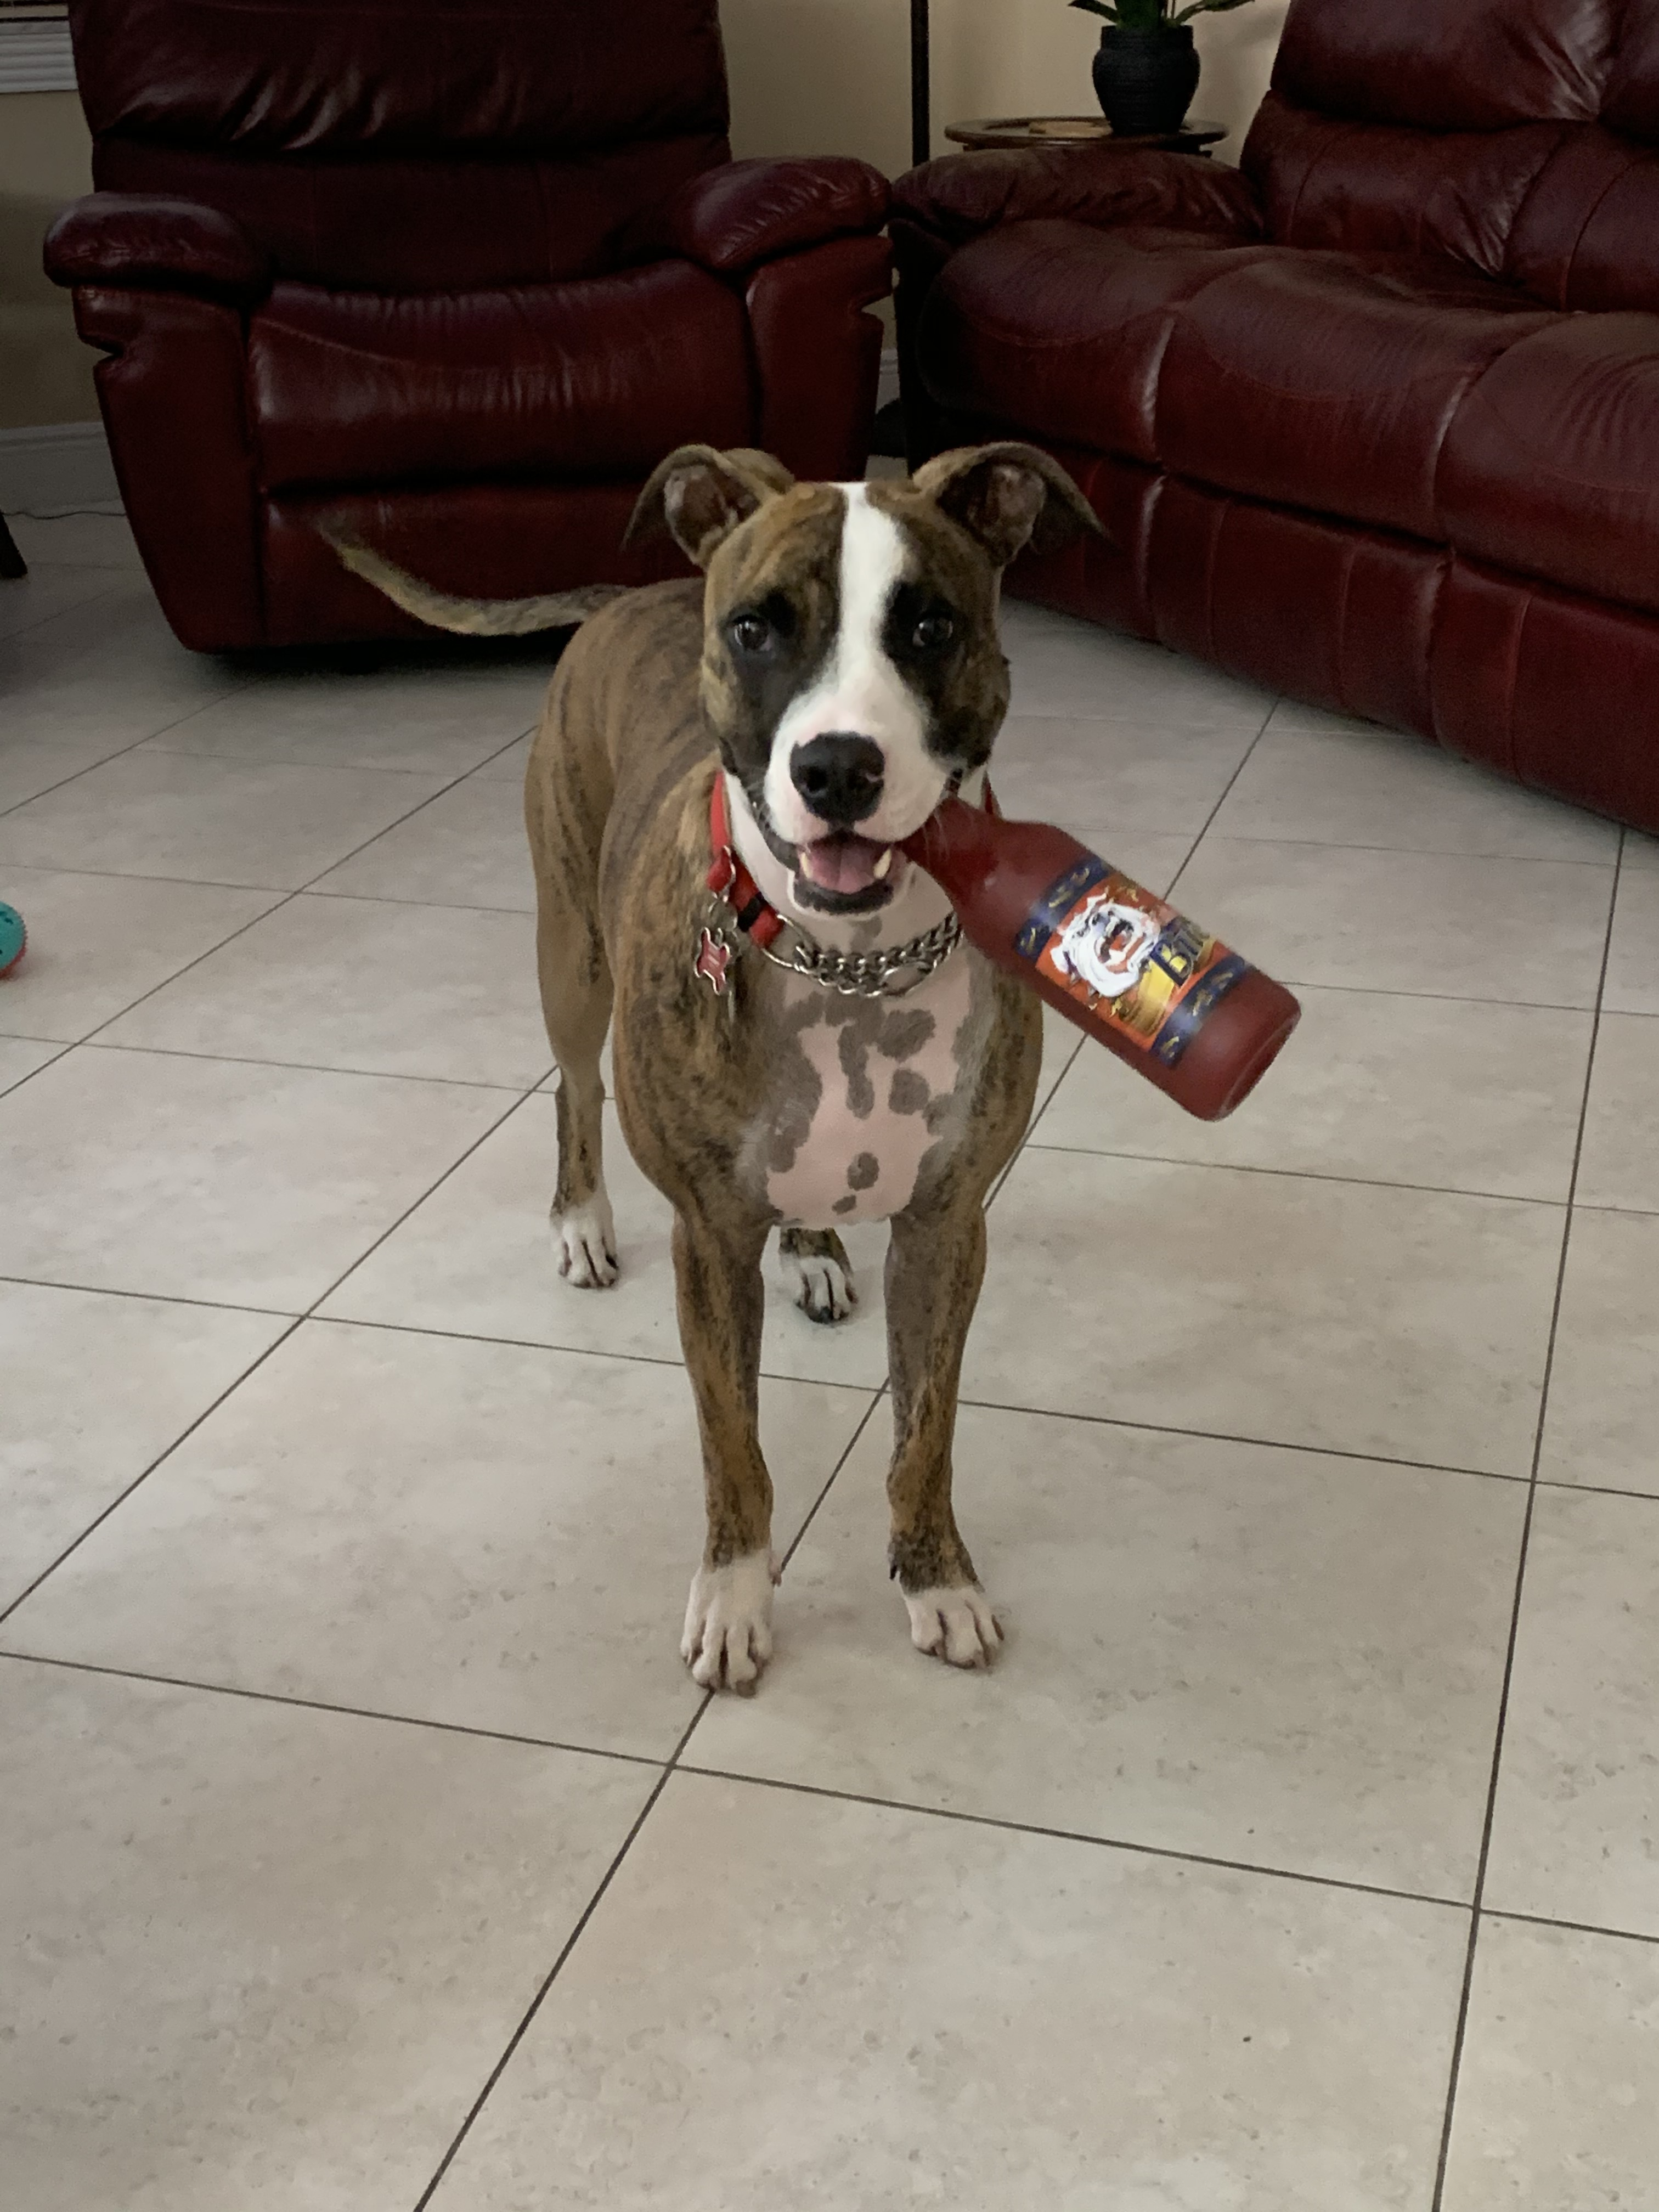
\includegraphics[width=0.9\textwidth]{teddy.jpg}
			\end{center}
		\end{minipage}

		\newpage

\item A previous head TA, Lindsey DeMarchi, had a very athletic black cat named Kiki who liked to jump and swat at things. One day I watched Kiki jump straight up and swat at the peep-hole in her door, 150 cm off the floor.
	This means that Kiki can push herself off the ground with enough velocity to reach a height of 150 cm. {\it (Note that this velocity is a property of Kiki herself; no matter where we take Kiki, this velocity is the same.}

\begin{enumerate}
\item With what velocity must Kiki leave the ground in order to jump 150 cm high?
\item How long will she be in the air before she lands?
\end{enumerate}

\item Suppose that Lindsey now takes Kiki to an elevator, accelerating upward at $\alpha=2\, \rm m/\rm s^2$. Kiki jumps up and tries to swat at one of the elevator buttons. This elevator button is 135 cm above the floor of the 
	elevator.

\begin{enumerate}
\item If Kiki jumps as high as she can, will she be able to push the button? How far above the elevator floor will she make it?
\item How long will Kiki be in the air?
\end{enumerate}

{\it Hint: Think very carefully about your coordinate system, and all of the consequences of the accelerating elevator. You may need the quadratic formula for this problem. If you are still stuck, draw position vs. time graphs for 
		both Kiki and the elevator button the wall she is trying to push.}

%\item Lindsey then travels to the planet Twilo with Kiki, which is quite Earthlike except for its value of $g=11.8\, \rm m/\rm s^2.$
%
%\begin{enumerate}
%\item How high can Kiki jump on Twilo?
%\item Based on a comparison of the last two problems, can you make any statements regarding gravity and acceleration?
%\end{enumerate}
%
%\item An object's position is given by the vector 
%
%$$\vec s(t) = (3\,\rm m/\rm s^3) t^3 \hat i + (4\, \rm m/\rm s^2) t^2 \hat j + (8\, \rm m/\rm s) t\hat k.$$
%
%\begin{enumerate}
%\item What is its velocity as a function of time?
%\item What is its acceleration as a function of time?
%\item Where is it at $t=10$ s?
%\end{enumerate}
%
%\item An object's position is given by the vector 
%
%$$\vec s(t) = (2\, \rm m) \cos (\omega t) \hat i + (2\, \rm m) \sin (\omega t) \hat j$$
%
%where $\omega = 1$ radian per second.
%
%\begin{enumerate}
%\item How would you describe this object's motion? 
%\item Hint: if you are stuck, compute and graph its position in the Cartesian plane at a variety of values of t (say, for integers 0-6).
%\end{enumerate}

\item A hiker is standing on the top of a mountain with a slope of 45 degrees. They kick a rock horizontally off of the top of the mountain at an initial speed $v_0$; it sails through the air until it lands 
	lower on the slope.

	\begin{enumerate}
		\item Think very carefully about how you can describe ``The rock lands back on the slope'' in mathematical terms. It will help to draw a picture, as always.
		\item Where on the slope does the rock land?
	\end{enumerate}

\end{enumerate}
\end{document}

